% Şekil: ticari bir eviricinin sabah devreye girişindeki güç--akım THD kaydı (Tablo tab:ticari-evirici-thd).
% Veri: tez-matlab-simulink/results/chapter2_profiles/legacy_commercial_inverter_record.csv
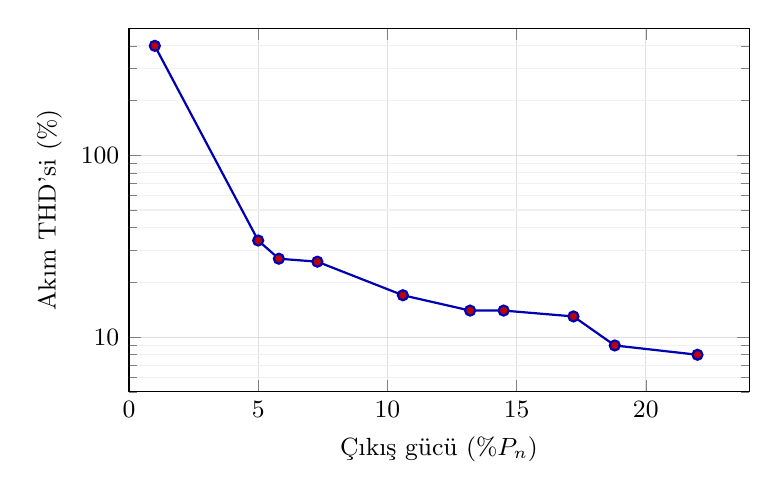
\begin{tikzpicture}
\begin{semilogyaxis}[
  width=0.78\textwidth, height=62mm,
  tick label style={font=\fontsize{9}{10.5}\selectfont}, label style={font=\fontsize{9}{10.5}\selectfont},
  xlabel={Çıkış gücü (\%$P_n$)}, ylabel={Akım THD'si (\%)},
  xmin=0, xmax=24, ymin=5, ymax=500,
  grid=both, grid style={gray!25}, minor grid style={gray!12},
  log basis y=10, log ticks with fixed point, /pgf/number format/use comma,
]
  \addplot[blue!70!black, thick, mark=*, mark size=1.8pt, mark options={fill=red!75!black}] coordinates {
    (1,400) (5,34) (5.8,27) (7.29,26) (10.6,17) (13.2,14) (14.5,14) (17.2,13) (18.8,9) (22,8)};
\end{semilogyaxis}
\end{tikzpicture}
